\section{Stochastic Programming}

\subsection{Motivation}

In this chapter we will explore optimization under uncertainty; in other words,
linear programming where some of our decision variables are stochastic.

We begin with a small example where a steel mill must plan a production schedule
to cater for future demand.

As production of the steel takes 3 months, the future market demand at $t=0$ is 
not known. However, the firm must allocate the right amount of resources for
mining and treating ore now.

\subsection{Feasibility Sets}\label{sec:spforms}

For the first stage:

\[
K_1 = \{ \bx \geq 0 : Ax = b \}
\]

Second stage \emph{elementary feasbility set}:

\[
K_2(\xi) = \{\bx : \mathscr{Q}(x,\xi) < \infty \} =  \{\bx : \exists \by \geq 0, \bW\by  = \bh - \bT\bx \}
\]

For continuous $\xi$ we define the \emph{possibility interpretation}:

\begin{alignat*}{2}
& K_2(\xi) = \{\bx : \mathscr{Q}(x) < \infty \} \\
& K_2^P(\xi) = \mathop{\cap}_{\xi \in \Xi} K_2(\xi) 
\end{alignat*}

$K_2 = K_2^P(\xi)$ holds when $\Xi$ is finite, as the following theorem states:

\begin{thm}\hfill\break
If $\Xi$ has finite second moments and $W$ is fixed, then $K_2 = K_2^p$
\end{thm}

\begin{proof}
For $K\subseteq K_2^p$, if $x \in K_2 \Rightarrow \mathscr{Q}(x) < \infty \Rightarrow 
\mathbb{E}_\xi\big[\mathcal{Q}(x,\xi)\big] < \infty \Rightarrow 
\underbrace{\mu (\mathcal{Q}(x,\xi)) = 2}_{\textrm{Probabilities sum to 1}}$.

We now have to show that $\{ \xi : \mathcal{Q}(x,\i)<\infty\}$ is a closed set.
\end{proof}

\begin{thm}\hfill\break
{\bf a)} For a given $\xi$, $K_2(\xi)$ is a convex polyhedron.\\
{\bf b)} When $\xi$ is a finite discrete random variable, $K_2$ is a convex polyhedron.
\end{thm}

\begin{proof}\hfill\break
{\bf a)} For some $x$ in the elementary feasbility set, that is,
\[
x \in K_2(\xi) = \big\{ x : \exists y \geq 0 : W y = h - Tx \big\}
\]

where the following is equivalent:

\[
h-Tx \in \text{pos}W = \big\{ t : \exists y \geq 0 : W y = t \big\}
\]

where pos$W$ is the positive cone of $W$. pos$W$ is a non-empty closed convex set, which
can be see since $0\in \text{pos}W$, \texttt{<insert closed/convex set proof>}, and it is
a cone since $\forall \lambda \in \mathbb{R}^{m_1}, t\in \text{pos}W \Rightarrow \lambda t \in
\text{pos}W$.\\

Due to the properties of pos$W$, we know that $\exists \{t : \sigma^\top t = \alpha\}$ such
that

\[
\sigma^\top (h-Tx) > \alpha
\]

and

\[
\text{pos}W \subseteq \{t : \sigma^\top t \leq \alpha\}
\]

Then, $0\in \text{pos}W \Rightarrow \alpha \geq 0$, and hence

\[
\sigma^\top (h-Tx) > \alpha \geq 0
\]

We prove by contradiction, i.e. if we can find $x$ such that $x\notin K_2(\xi)$ then
$h - Tx \notin \text{pos}W$. Then the separating hyperplane theorem tells us that we
can find a hyperplane $\big\{ t : \sigma^T t = \alpha \big\}$ such that

\[
h-Tx \in \big\{ t : \sigma^T t \geq \alpha \big\}
\]

and

\[
\text{pos}W \subseteq \big\{ t : \sigma^T t < \alpha \big\}
\]

However, because $\bm{0} \in \text{pos}W \Rightarrow \bm{0} \in \big\{ t : \sigma^T t < \alpha \big\}$
Therefore we must have that $\alpha > 0$.

Because $h-Tx$ is on the the other side of the cone we have $\sigma^T (h-Tx) \geq \alpha > 0$.


We now assume the opposite: $\exists t\in \text{pos}W : \sigma^T t\geq 0$. But
if $t\in \text{pos}W \Rightarrow \lambda t\in \text{pos}W \forall \lambda \in \mathcal{R}_n^+
\Rightarrow \lambda \sigma^T t \leq \alpha, \forall \lambda > 0$. This is a contradiction
because as $\lambda \rightarrow \infty, \lambda \sigma^T t < x$ cannot hold!
Therefore $\{ t: \sigma^T t = 0\}$ is a separating hyperplane!\\

Since there are be lots of separating hyperplanes $M = \{ \sigma : \forall t \in \text{pos}W :
\sigma^T t < 0\}$ this means that if $x\in K_2(\xi) \Leftrightarrow h-Tx \in \text{pos}W
\Leftrightarrow \sigma^T(h-Tx) < 0, \forall \sigma \in M$.

We arrive at the following conclusion: being in the elementary feasibility set means
being on the right side of all separating hyperplanes $\sigma \in M$.\\

$M$ is a non-empty convex cone: $\sigma^T (h-Tx) \leq 0, \forall \sigma \in M \Leftrightarrow
\sigma_i^T(h-Tx) < 0, i=1,..,|M|$.

Therefore, being in the elementary feasibility sets is the same as satisfying $|M|$ linear
inequalities, therefore $K_2$ is a polyhedron.
\end{proof}

\begin{proof}{\bf b)}
Let $\Xi = \{\xi_1, .., \xi_S\}$ (finite support) with $\prob{\xi(\omega)=\xi_s)} = p_s,\; s=1,..,S$.
$x\in K_2 \Leftrightarrow \mathcal{Q}(x) < \infty \Leftrightarrow \sum_{s=1}^S p_s
\mathcal{Q}(x,\xi_s) < \infty \Leftrightarrow \mathcal{Q}(x,\xi_s) < \infty, s=1,..,S
\Leftrightarrow x\in K_2(\xi_s), s=1,..,S = \cap_{s=1}^S K_2(\xi_s)$.
%The intersubsection of 
\end{proof}

Polyhedrons give rise to cutting-plane algorithms as we will see in subsection \ref{sec:lshape}.

The following theorem describes properties of the recourse function $\Q(x,\xi)$:

\begin{thm}\hfill\break
For a given $\xi$, $\Q(x,\xi)$ is\\
{\bf a)} piecewise linear convex in $(h,T)$.\\
{\bf b)} piecewise linear concave in $q$.\\
{\bf c)} piecewise linear convex in $x \forall x\in K_2$.
\end{thm}

\begin{proof}{\bf a)} and {\bf c)}\\

\end{proof}

\begin{proof}{\bf b)}
$\Q(x,\xi)$ = min $\{q^Ty : Wy = h-Tx, y\geq0 \}$
            = min $\{q^Ty_i : i=1,..,n\}$ where $y_i$ are the extreme points of $\{ y:  Wy = h-Tx, y\geq0 \}$ 
\end{proof}



\subsection{Formulations}

We will look at:

\begin{itemize}
\item First-order problems (use mean)
\item Second-order (scenarios)
\item Expected Value solution
\item EVPI
\item VSS
\end{itemize}

\subsubsection{Two-stage recourse problem}

This is the most basic type of stochastic program, namely where we only consider two stages
with fixed recourse (i.e. $\bm{W}$ is fixed).\\

\stone\\

Determine first-stage variable $\bx$.\\

\obs\\

$\xi(\omega)$\\

\sttwo\\

Make second-stage decisions based on the new information.\\

\form\\

This is an \emph{deterministic equivalent}:

\begin{alignat*}{2}
\textrm{min} & \quad \bm{c}^T \bx + \mathbb{E}_\xi \Big[\text{min } q(\omega)^Ty(\omega)\Big] \ & \ \\
\text{s.t.}  & \quad \bm{Ax} = \bm{b} & \ \\
             & \quad  \bm{T}(\omega)\bx + \bm{W}y(\omega) = h(\omega), & \ \\
             & \quad \quad x \in \mathcal{X} & \
\end{alignat*}

The first constraint represents the deicison we made in the first stage, while the
second constraint links the first and second stages.

\subsubsection{Multistage recourse problem}

\textbf{Implicit form}

\[
\text{min} \{ c^T x + \mathbb{E}_\xi \Q(x,\xi) : Ax=b, x\in X \}
\]

where $\xi$ is the random vector containgin the information we observe in the
second stage and

%\marginnote{The right-most expression is a probability-weighted sum!}
\[
\Q(x, \xi) = \text{min} \{ q^T y : Wy = h - Tx, y \geq 0 \}
           %= \sum_{s=1}^S p_s \Q^s(x)
\]

A more condensed implicit representation:

\[
\text{min} \{ c^T x + \mathscr{Q}(x) : Ax=b, x\in X \}
\]

where $\mathscr{Q}(x) = \mathbb{E}_\xi \Q(x,\xi)$.

This formulation is also called the \emph{deterministic equivalent}, since we
can compute the expectation in the first stage.

\textbf{Extensive form}

Assume that $\xi$ has a discrete distribution with finite support $\Xi = \{\xi_1, .., \xi_S\}$
such that

\[
\mathcal{P}\big[\xi(\omega) = \xi_s\big] = p_s,\quad \quad s=1..S
\]

\begin{alignat}{2}
\textrm{max} & \quad \bm{c}^T \bx + \mathbb{E}_{\xi_2}\Big[\text{min }c^2(\omega)^\top x^2(\omega) + \ldots + \mathbb{E}_{\xi_T}\big[
\text{min }c^T(\omega)^\top x^T(\omega) \big]\ldots\Big]& \ \\
\text{s.t.}  & \quad \bm{T}_1^s x_1^s = \bm{b}_1, \quad \quad s=1..S\ \\
             & \quad \bm{T}_{t-1}^s \bx_{t-1}^s + \bm{W}_t x_t^s = h_t^s, \quad \quad s=1..S\ \\
             & \quad \quad x_t^s = x_t^{s'}, \qquad \text{if } \big[ \xi_1^s, ..., \xi_t^s \big] = \big[ \xi_1^{s'}, ..., \xi_t^{s'} \big], t=2..T, s=1..S \ \label{eq:nonanti} \\
             & \quad \quad x_1^s \in \mathcal{X}_1, .. x_t^s \in \mathcal{X}_T & \ \\
\end{alignat}

This is a solvable linear program, but it is quite large due to the number of constraints.

\textbf{General Formulation}

Given the probability space $(\Omega, \mathcal{F}, \{ \mathcal{F}_{t} \}_{t=1}^T, \mathcal{P})$ 
with $\mathcal{F}_t \subseteq \mathcal{F}_{t+1}$ where $\mathcal{F}_1 = \emptyset$, 
$\mathcal{F}_T = \mathcal{F}$ we can formulate a multi-stage recourse problem as follows:

\begin{alignat}{2}
\textrm{max} & c_1 x_1 +  & \\
\text{s.t.}  & \quad \bm{T}_1^s x_1^s = \bm{b}_1, & \quad \quad s=1..S\ \\
             & \quad \quad x_1^s \in \mathcal{X}_1, .. x_t^s \in \mathcal{X}_T & \ \\
\end{alignat}

\textbf{Nodal formulation}

A nodal formulation use \emph{scenario trees}, as depicted in figure \ref{fig:stex}.

% Set the overall layout of the tree
\tikzstyle{level 1}=[level distance=3.5cm, sibling distance=3.5cm]
\tikzstyle{level 2}=[level distance=3.5cm, sibling distance=2cm]
\tikzstyle{circ} = [circle, minimum width=3pt,fill, inner sep=0pt]
\begin{figure}[h!]
\begin{center}
\begin{tikzpicture}[grow=right, sloped]
\node[circ] {}
    child {
        node[circ] {}        
            child {
                node[circ, label=right:
                    {$s_4$}] {}
                edge from parent
                %node[above] {$W$}
                %node[below]  {$\frac{4}{9}$}
            }
            child {
                node[circ, label=right:
                    {$s_3$}] {}
                edge from parent
                %node[above] {$B$}
                %node[below]  {$\frac{5}{9}$}
            }
            edge from parent 
            %node[above] {$W$}
            %node[below]  {$\frac{4}{7}$}
    }
    child {
        node[circ] {}
        child {
                node[circ, label=right:
                    {$s_2$}] {}
                edge from parent
                %node[above] {$B$}
                %node[below]  {$\frac{3}{9}$}
            }
            child {
                node[circ, label=right:
                    {$s_1$}] {}
                edge from parent
                %node[above] {$W$}
                %node[below]  {$\frac{6}{9}$}
            }
        edge from parent         
            %node[above] {$B$}
            %node[below]  {$\frac{3}{7}$}
    };
\end{tikzpicture}
\end{center}
\caption{An example of a scenario tree.}
\label{fig:stex}
\end{figure}

\begin{itemize}
\item $\mathcal{N}$ : nodes
\item $o$ : root
\item $\mathcal{N}_+(n)$ : successors of node $n$
\item $p^{n/n-}$ : transition probability
\item $p^n$ : probability of being in $n$, $\; p^n = p^{n-} p^{n/n-}, \quad n \in \mathcal{N} \setminus \{0\}$ 
\end{itemize}

Such a formulation obviates the need for non-anticipativity constraints since we always know the predecessor
node $n^-$.

W have $m|N|$ constraints and $n|N|$ variables.

\subsubsection{Chance Constrained Formulation}

Assuming we know the distribution of the underlying scenarios we may formulate the
probability in terms of quantiles. Consider the following example the UFL problem with
stochastic demand; i.e. $\xi = \{d_1, .., d_j\}$.

\begin{alignat*}{2}
\textrm{max} & \quad \bm{c}^T \bx + \sum_{j=1}^m \sum_{i=1}^n q_{ij} y_{ij}\ & \ \\
\text{s.t.}  & \quad\; y_{ij} \leq M x_j \ & \quad \quad j = 1..m, i = 1..n\ \\
             & \quad \prob{\sum_{j=1}^m y_{ij} \geq d_i(\omega)} \geq \alpha_i \ & \quad \quad i=1..n \\
             & \quad \quad x \in \mathcal{B}^1, y_{ij} \geq 0, \ & \quad \quad j = 1..m, i = 1..n
\end{alignat*}

\subsubsection{Elimination of Recourse Variables}

Assume $W = [I,-I]$, $q^T = ((q^+)^T, ((q^-)^T)$ and $y^T = ((y^+)^T, ((y^-)^T)$.\\

{\it First stage}:

\[
min \{ c^T x + \mathcal{Q}(x) : Ax=b, x\in X\}
\]

{\it Second stage} (we make the assumption that it is linear)

\[
\mathcal{Q}(x) = \mathbb{E}_{\xi}\big[ \mathcal{Q} x, \xi(\omega) \big]
\]
\[
\mathcal{Q}(x) = \text{min} \{\bq^+(\omega)\by^+ + \bq^-(\omega)\by^- : \by^+ - \by^- = \bm{h}(\omega) - \bm{T}(\omega)\bx, \by^+, \by^- \geq 0 \}
\]

Now, since nothing links the $\by$ variables we may decompose the minimization problem
above to a sum:

\[
= \sum_{i=1}^{n_2} \text{min} \{q_i^+(\omega)y_i^+ + q_i^-(\omega)y_i^- : y_i^+ - y_i^- = h_i(\omega) - \bm{T}_i(\omega)\bx, y_i^+, y_i^- \geq 0 \}
\]


Taking the example from before, the random recourse variables $y^+$ and $y^-$ are
complementary\footnote{Check definition from Trine's article!}, meaning that $y^+ y^- = 0$.i
We substitute the random recourse varibles:

\[
= \sum_{i=1}^{n_2} \{q_i^+(\omega)[h_i(\omega) - \bm{T}_i(w)x]^+ + q_i^-(\omega)[\bm{T}_i(w)x - h_i(w)]^+ : q_i^+(\omega) + q_i^-(\omega) \geq 0 \}
\]

\subsubsection{Second-stage Integer Variables}

Paper to \LaTeX is marked \# 1313

\subsubsection{Example: UFL}

The uncapacitated facility location problem is an example of a simple recourse problem.
The random vector $\xi$ is defined as follows:

%\[
%\bm{\xi} = (\bm{v, r, t_1, ..., t_m, d)}
%\]

where

\begin{itemize}
\item $\bm{v}:$ variable cost vector
\item $\bm{r}:$ price vector
\item $\bm{t}:$ transportation cost for each customer $i=1..m$
\item $\bm{d}:$ demand vector
\end{itemize}

\stone\\

Determine $x_j$, $y_{ij}$ (opening facilities and distribution).\\

\obs\\

$\bm{v_j(\omega), r_j(\omega), t_{ij}(\omega),d_j(\omega)}$\\

\sttwo\\

Based on the realization of $\xi$ we can now determine the shortages
and surplusses at each customer denoted by $w_i^+(\omega)$ and $w_i^-(\omega)$,
respectively.\\

\form

\begin{alignat*}{2}
\textrm{max}  & \quad  -\sum_{j=1}^m c_j x_j + \mathbb{E}_\xi \Big[\sum_{j=1}^{m} \sum_{i=1}^{n} (v_j(\omega) + t_{ij}(\omega))y_{ij})\Big] + \mathbb{E}_\xi \Big[\sum_{i=1}^n r_i(\omega)d_i(\omega)\Big]\ \\
 & \quad - \mathbb{E}_\xi \Big[\sum_{i=1}^n q_i^+ w_i^+(\omega) + q_i^- w_i^-(\omega)\Big]\ \\
\text{s.t.} & \quad \quad \sum_{j=1}^m y_{ij} + w_i^+(\omega) - w_i^-(\omega) = d_i(\omega),\ & i = 1..n\ \\
            & \quad \quad y_{ij} \leq M x_{ij}, & j=1..m, \; i = 1..n \ \\
            & \quad \quad x_j \in \mathcal{B}^1, y_{ij}, w_i^+, w_i^- \geq 0 & \
%\text{s.t.} & \quad \sum_{i=1}^m a_{ij} + e_j t_j \geq g_j &,\ & 1\leq j\leq n\\
\end{alignat*}

The recourse variables in in the programme above are $w_i^+$ and $w_i^-$. By observing that 

\[
w_i^+ = \mathbb{E}_\xi \Big[ d_i(\omega) + \sum_{j=1}^m y_{ij} \Big]^+
\]

and

\[
w_i^- = \mathbb{E}_\xi \Big[\sum_{j=1}^m y_{ij} - d_i(\omega) \Big]^+
\]

we may eliminate the recourse variables by substitution (also called \emph{simple recourse}):

\begin{alignat*}{2}
\textrm{max}  & \quad  -\sum_{j=1}^m c_j x_j + \mathbb{E}_\xi \Big[\sum_{j=1}^{m} \sum_{i=1}^{n} (v_j(\omega) + t_{ij}(\omega))y_{ij})\Big] + \mathbb{E}_\xi \Big[\sum_{i=1}^n r_i(\omega)d_i(\omega)\Big]\ \\
 & \quad - \Big[\sum_{i=1}^n q_i^+ \mathbb{E}_\xi \Big[ d_i(\omega) + \sum_{j=1}^m y_{ij} \Big]^+ + q_i^- \mathbb{E}_\xi \Big[\sum_{j=1}^m y_{ij} - d_i(\omega) \Big] \Big]\ \\
\text{s.t.} & \quad \quad \sum_{j=1}^m y_{ij} = d_i(\omega),\ & i = 1..n\ \\
            & \quad \quad y_{ij} \leq M x_{ij}, & j=1..m, \; i = 1..n \ \\
            & \quad \quad x_j \in \mathcal{B}^1, y_{ij}, w_i^+, w_i^- \geq 0 & \
\end{alignat*}

We say that the problem exhibits \emph{simple} recourse when we can eliminate
variables in this manner.

\subsection{Value of Stochastic Programming}

For a given stochastic programing problem, we have four different ways of solving
the problem:

\[
RP : \textrm{min  } \mathbb{E}_\xi{\big[z(x,\xi)\big]}, \; x \in K_1 \cap K_2(\xi)
\]

\[
WS : \mathbb{E}_\xi \big[\textrm{min }_x z(x, \xi) \big]
 %= \mathbb{E}{\big[\textrm{min  } z(\overline{x}(\overline{\xi}), \xi)\big]}
\]

\[
EV : \textrm{min  } z(x, (\overline{\xi})), \quad \mathbb{E}\big[\xi\big] = \overline{\xi}
\]

For the $EV$, we still have the recourse problem, we just do not care about the
stochasticity.

We also have the Expected Value of the $EV$:

\[
EEV : \mathbb{E}\big[ z(\overline{x}(\overline{\xi}), \xi) \big]
\]

The following proposition shows their relationship:

\begin{proposition}
$WS \leq RP \leq EEV$
\end{proposition}

\begin{proof}
We always have $z(\overline{x}(\xi), \xi) \leq z(x^*, \xi)$ regardless of $\xi$. Taking
the expectation on both sides shows the first inequality. 

For $RP\leq EEV$, it is clear that $\textrm{min  }_{x \in K_1 \cap K_2(\xi)} \mathbb{E}_\xi{\big[z(x,\xi)\big]}
\leq \mathbb{E}_\xi \big[z(\overline{x}(\overline{\xi}), \xi)\big]$.
If $\overline{x}(\overline{\xi})\notin K_2$, the recourse function takes on the value
$\infty$, so the inequality still holds.
\end{proof}

\begin{proposition}
If $q,\; W,\; T$ are fixed, then $EV \leq WS$.
\end{proposition}

\begin{proof}
Let $f(\xi) = \textrm{min}_{x\in K_1 \cap K_2(\xi)}$. $f$ is convex in $\xi$ because we
have already proved that $f$ is convex in its RHS.\\
By Jensen's inequality we have:

\[
\mathbb{E}_\xi \big[f(\xi)\big] \geq f(\mathbb{E}_\xi\big[\xi\big])
\Leftrightarrow WS \geq EV
\]

\end{proof}

We now define the \emph{expected value of perfect information} (EVPI) and \emph{value of
the stochastic program} (VSS) as the distances between the above formulations in terms
of objective value, so as to assess their utility.

\[
EVPI = RP - WS
\]

\[
VSS = EEV - RP
\]

We assume $EVPI, VSS \geq 0$.
Figure \ref{fig:valuesofsp} shows the relationship between these problems graphically.

\begin{figure}[h!]
\begin{center}
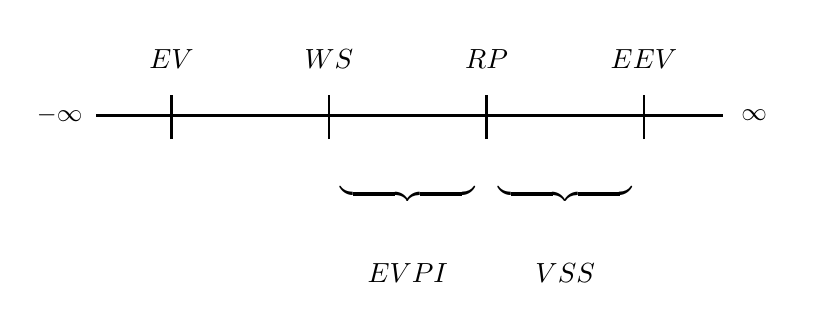
\begin{tikzpicture}[-,shorten >=1pt,auto,node distance=1.5cm,thick,minimum size=0.8cm,main node/.style={circle,draw=red,very thick}]
\tikzstyle{selected edge} = [draw,line width=6pt,-,blue!30]
\coordinate (origo) at (0,0);
\coordinate (EV) at (0,1);
\coordinate (WS) at (0,3);
\coordinate (RP) at (0,5);
\coordinate (EEV) at (0,7);

% Draw axes
\draw[-] (8,0) -- (origo) node[left] {\small $-\infty$};
\draw[-] (1,-0.3) -- (1,0.3) node[above] {$EV$};
\draw[-] (3,-0.3) -- (3,0.3) node[above] {$WS$};
\draw[-] (5,-0.3) -- (5,0.3) node[above] {$RP$};
\draw[-] (7,-0.3) -- (7,0.3) node[above] {$EEV$};
\node[] at (8.4,0) {\small $\infty$};

\node[] at (4,-1) {$\underbrace{\phantom{\hspace{1.7cm}}}$};
\node[] at (4,-2) {$EVPI$};

\node[] at (6,-1) {$\underbrace{\phantom{\hspace{1.7cm}}}$};
\node[] at (6,-2) {$VSS$};

\end{tikzpicture}
\caption{Relationship between $EV$, $WS$, $RP$ and $EEV$ for a minimization problem with fixed $q$, $W$ and $T$.}
\label{fig:valuesofsp}
\end{center}
\end{figure}

\subsubsection{Example}

Observe the following two-stage stochastic program\footnote{For ease of exposition I 
will use colours to keep track of what variables go where.} :

\[
\textrm{min } \{ 6x + \mathcal{Q}(x) : x\geq 0 \}
\]

where

\[
\mathcal{Q}(x) = \textrm{min } \{ 10y, y \geq x-\xi, y \geq \xi-x \}
\]

and $\textcolor{blue}{\xi_1} = \textcolor{blue}{\frac{1}{3}}$, $\textcolor{blue}{\xi_2} = 
\textcolor{blue}{\frac{2}{3}}$, $\textcolor{purple}{p_1} = \textcolor{purple}{\frac{1}{2}}$
and $\textcolor{purple}{p_2} = \textcolor{purple}{\frac{1}{2}}$.\\

\textbf{Computing $WS$}

For each $\xi$:

\[
\textrm{min } \{ 6x + 10|x-\textcolor{blue}{\frac{1}{3}}|: x\geq 0 \} = 2,\;\; 
\overline{x}(\textcolor{blue}{\frac{1}{3}}) = \frac{1}{3}
\]

\[
\textrm{min } \{ 6x + 10|x-\textcolor{blue}{\frac{2}{3}}|: x\geq 0 \} = 2,\;\; 
\overline{x}(\textcolor{blue}{\frac{2}{3}}) = \frac{2}{3}
\]

$WS = \textcolor{purple}{\frac{1}{2}}\cdot 2 + \textcolor{purple}{\frac{1}{2}}\cdot 4 = 3$

\textbf{Computing $EV$}

$\mathbb{E}\big[\xi\big]= \textcolor{purple}{\frac{1}{2}}\cdot \textcolor{blue}{\frac{1}{3}} 
+ \textcolor{purple}{\frac{1}{2}}\cdot \textcolor{blue}{\frac{2}{3}} = \textcolor{orange}{\frac{1}{2}}$

\[
\textrm{min } \{ 6x + 10|x-\textcolor{orange}{\frac{1}{2}}|: x\geq 0 \} = 3,\;\; 
\overline{x}(\textcolor{orange}{\frac{1}{2}}) = \textcolor{red}{\frac{1}{2}}
\]

\textbf{Computing $EEV$}

\begin{alignat*}{2}
EEV & = \textcolor{purple}{\frac{1}{2}}\big(6 \textcolor{orange}{\frac{1}{2}} + 10|\textcolor{orange}{\frac{1}{2}} - \textcolor{blue}{\frac{1}{3}}|) \\
& + \textcolor{purple}{\frac{1}{2}}\big(6 \textcolor{orange}{\frac{1}{2}} + 10|\textcolor{orange}{\frac{1}{2}} - \textcolor{blue}{\frac{2}{3}}|) \\
& = 4\frac{2}{3}
\end{alignat*}

\textbf{Computing $RP$}

\begin{alignat*}{2}
RP & = \textrm{min } \{ 6x + \textcolor{purple}{\frac{1}{2}}\big(10|\textcolor{red}{\frac{1}{2}} - \textcolor{blue}{\frac{1}{3}}|)
+ \textcolor{purple}{\frac{1}{2}}\big(10|\textcolor{red}{\frac{1}{2}} - \textcolor{blue}{\frac{2}{3}}|)\} \\
& = 3\frac{2}{3},\;\; x^* = \frac{1}{3}
\end{alignat*}

\subsection{Scenario Generation}

This subsections discusses different ways of generating data for input to our
stochastic programs. Also, it is often convenient for our input variables to
have certain statistical properties (moments).

\subsubsection{Moment Matching}

Moment matching is a way of generating these input data by solving a nonlinear
program that minimizes the square error of our realizations against the moments
we wish to match.

\begin{alignat*}{2}
\textrm{min}& \quad \quad \sum_{V_s} w_i \big[ f_i(\xi, p) - V_i \big]^2 \ \\
\text{s.t.} & \quad \quad \sum_{s=1}^S p_s = 1 & \ \\
            & \quad \quad p_s \geq 0, \; s=1..S & \
\end{alignat*}

where $w_i$ are weights e.g. a higher value of $w_i$ will cause an NLP solver to
minimize the error for the moment even more.\\

{\large\bf Pros \& Cons of Moment Matching:}
\begin{itemize}
\item[-] One large non-convex program is hard to solve
\item[-] How do we model dependencies between nodes?
\item[-] Might not produce the optimal solution
\item[-] Inconsistencies in probabilities due to datasets differing in size
\item[+] Independent of the size of the data set
\item[+] No knowlege of $\xi$ assumed
\item[+] Under/overspecification of $\xi$
\item[+] Weights = "faith"
\end{itemize}

If the number of moments and the numer of scenarios match, moment matching typically
performs well. If we were to increase the number of moments we wished to match, we 
would at some point \emph{overspecify} the distribution,. An example could be that that
we would not have enough variables to fully represent the covariance in the
distribution.\\

On the other hand, if we required more scenarios than moments, for instance
only matching the first moment for a larger number of scenarios, we could risk 
that every scenario except one that attains the mean value with probability one.

\subsubsection{Sampling Methods}

The solution to

\[
\hat{z} = \textrm{min}_{x \in \mathbb{X}} \frac{1}{S}\sum_{s=1}^S z(x,\xi_s)
\]

is called the \emph{sample average approximation}. If $\xi_1,..,\xi_S$ are i.i.d.,
then by the Law of Large Numbers:

\[
\hat{z} = \textrm{min}_{x\in \mathbb{X}} \frac{1}{S}\sum_{s=1}^S z(x,\xi_s) \rightarrow \mathbb{E}_\xi \big[z(x,\xi)\big]
\]

{\large\bf Pros \& Cons of Sampling:}
\begin{itemize}
\item[-] Many samples required, large SP, harder to solve ($S^N$ scenarios is $\xi \in \mathbb{R}^N$)
\end{itemize}

\subsubsection{Scenario Reduction}

Since the amount of nodes required for non-trivial problems increases exponentially
in the amount of stages, it is convenient to reduce this amount to make the problem
computationally tractable. As we will see, we may delete a subset of the initial set
of nodes $I = \{1, .., S\}$ in a methodical way. This subsection is dedicated to scenario
reduction which address the following question:\\

\begin{center}
Given $I = \{1, .., S\}$ of initial scenarios, which ones do we chose to delete?
\end{center}

In other words, we seek to find $J \subset I$.


\begin{alignat}{1}
P_d: d(I, q) = \text{min} \Big\{\sum_{i\in I} \sum_{j\notin J} c_{ij} \eta_{ij} : \eta_{ij} \geq 0, \;\sum_{j\notin J} \eta_{ij} = p_i, \;\sum_{i\in I} \eta_{ij} = q_j, i \in I, j \notin J \Big\}
\label{eq:distanceprimal}
\end{alignat}


If we fix the cardinality $k = |J|$, we solve the scenario reduction problem using the
following algorithm:\\

\begin{enumerate}
\item Compute distances between scenarios 
\item Chose scenarios to deleted based on distances (and previous choices)
\item Redistribute probabilities
\end{enumerate}


\begin{thm}\hfill\break
Given $J \subset I$, 

\[
D_j = \text{min  } \{ d(J, q) : \sum_{j \notin S} q_j = 1, q_j \geq 0,
j \notin J \} = \sum_{i\in J} p_i \textrm{min }_{k\notin J} c_{ik}
\]

where $S$ is the set of scenarios, and $I$ is the set of scenarios we keep, with
optimal solution:

\[
q_j^{*} = p_j + \sum_{i \in J \cap J_j} p_i, \quad j\notin J
\]

where $ J_j = \{ i \in I : c_{ij} = \text{min  }_{k \notin J} c_{ik} \}$.
\end{thm}

\begin{proof}
We find upper and lower bounds for $D_j$ and see that the values for $q_j$ coincide
for fixed $J$.\\

We first take the dual of $P_d$ (\ref{eq:distanceprimal}):

\[
d(J, q) = \text{max  } \{\sum_{i\in I} p_i u_i + \sum_{j\notin J} q_jv_j : u_i+v_j \leq c_{ij}, i\in I, j\notin J \}
%\overline{v}_j=0, \
\]

We try to construct a feasible solution:\\
Let $\overline{u}_i = \text{min  }_{k\notin J} c_{ik}, \overline{v}_j=0, i\in I, j\notin J$\\
Clearly, $\overline{u}_i \leq c_{ij}$!
So a feasible solution is:

\[
\overline{u}_i  = \text{min  }_{k\notin J} c_{ik}
\]

\[
\overline{v}_j = 0
\]

If we insert this feasible solution:

\[
d(J,q) \geq \sum_{i\in I} p_i \text{min}_{k\in J} c_{ik} = \sum_{i\in J} p_i \text{min}_{k\in J} c_{ik}
\]

The last equality holds because the distance from the set $I$ to itself is zero. This holds for all $q$,
therefore also the $q$ that minimizes the distance i.e. the optimal value to the reduction problem has
the same lower bound:\\

\[
D_j \geq \sum_{i\in J} p_i \text{min}_{k\notin J} c_{ik}
\]

We now construct a feasible \emph{primal} solution for 

\begin{center}
$\eta_{ij} =
\begin{cases}
p_i & i\in J\cap J_j \;\text{ or }\; i=j, i\in I, j\notin J\\
  0 & 
\end{cases}$
\end{center}

and

\[
q_j = p_j + \sum_{i\in J \cap J_j} p_i,\quad j\notin J
\]

We must now show that this solution satisfies the following constraints:\\

\begin{enumerate}
\item $\overline{\eta}_{ij} \geq 0, i \in I, j\notin J$
\item $\sum_{j\notin J} \overline{\eta}_{ij} =
\begin{cases}
\overline{\eta}_{ik} & i\in J\cap J_k \;\text{ for some  }\; k\notin J\\
\overline{\eta}_{ii} & i\notin J
\end{cases}$
\item $\sum_{i\in I} \eta_{ij} = q_j$
\end{enumerate}

The first is trivially satisfied, and both piecewise constraints equate to $p_i$ by 
defition.
For the third we observe the following:\\

\[
\sum_{i\in I} \eta_{ij} = p_j + \sum_{i\in J\cap J_j} p_j = \overline{q}_j
\]

This is \emph{exactly} the definition, and is therefore a feasible solution. Hence,
we have an upper bound:

\begin{alignat*}{2}
d(J, \overline{q}) \leq \sum_{i\in I} \sum_{j\notin J} c_{ij} \overline{\eta}_{ij}
= \underbrace{\sum_{i \notin J}\sum_{j\notin J} c_{ij} \overline{\eta}_{ij}}_{\text{Keep}}
+ \underbrace{\sum_{i \in J}\sum_{j\notin J} c_{ij} \overline{\eta}_{ij}}_{\text{Goes away}} & \\
= \underbrace{\sum_{i\notin J} c_{ij} \overline{\eta}_{ij}}_{\text{distance from $I$ to $I$ = 0}}
+ \underbrace{\sum_{j\in J} p_i \text{min}_{k\notin J} c_{ik}}_{\text{Take the closest}}
= \sum_{j\in J} p_i \text{min}_{k\notin J} c_{ik}
\end{alignat*}

Now we just need to check if $\overline{q}_j \geq 0$ (given) sum to one:

\begin{alignat*}{2}
\sum_{j\notin J} q_j = \sum_{j\notin J} p_j + &\sum_{j\notin J} \sum_{i\in J\cap J_j}p_i\\
= \sum_{j\notin J} p_j + \underbrace{\sum_{i\in J} p_i}_{\text{=0}} & \\
= \underbrace{\sum_{j\notin J} p_j = 1}_{\text{From the definition}} &
\end{alignat*}

Thus we have proved that

\[
D_j \leq d(J,\overline{q}) \leq \sum_{i \in J} p_i\; \text{min}_{k\notin J} c_{ik}
\]

and we have a lower bound.
\end{proof}

So far, we have seen how to \_\_\_\_\_\_\_\_. We now go through how to select the
set $J\subset I$!

Given $D_j \forall J\subset I$, the reduction problem looks as follows:

\begin{equation}\label{eq:redprob}
D=\text{min} \big\{ \sum_{i\in J} p_i \text{min }_{k\notin J} c_{ik} : J\subseteq I, \left\vert{J}\right\vert = k\big\}
\end{equation}

In the following, let $J=\{l_1, .., l_k\}$ so the reduction problem is:

\begin{equation}
D=\text{min} \big\{ \sum_{i\in J} p_i \text{min }_{l\neq k} c_{ik} : l\in I \big\}
\end{equation}

As we saw, if we have an optimal solution $l^*$ we can easily redistribute the probabilites.

\begin{thm}
$\sum_{i=1}^k p_{l_i} \text{min}_{k\neq l_i} c_{ik} \leq D_k,\; i=1,..,k$
is a lower bound
\end{thm}

\begin{proof}
Let $J= \{j_1, .., j_j\}$, $|J| = k$, by theorem (link above):

\begin{alignat*}{2}
D_j = \sum_{i\in J} p_i \text{min}_{k\notin J} c_{ik} & = \sum_{i=1}^k p_i \text{min}_{k\in \{j_1, .., j_k\}} c_{ik}\\
& = \underbrace{\sum_{i=1}^k p_{j_i} \text{min}_{k \neq j_i} c_{j_i k}}_{\text{larger feasible region}} \\
& = \underbrace{\sum_{i=1}^k p_{l_i} \text{min}_{k \neq l_i} c_{l_i k}}_{\text{independent of } J}
\end{alignat*}

So it is a lower bound for \emph{any} $J$ (= $D_j$) , even the one that minimizes (= $D$)!
Hence

\[
D \geq \sum_{i=1}^k p_{l_i} \text{min}_{k\neq l_i} c_{l_i k}
\]
\end{proof}

So if for $i=1,..,k$, $\text{min}_{k\neq l_i} c_{l_i k}$ has an optimal solution $J=I\setminus \{l_1,..,l_k\}$,
then 

\[
D_j \geq \sum_{i=1}^k p_{l_i} \text{min }_{k\neq l_i} c_{l_i k}
= \sum_{i=1}^k p_{l_i} \text{min}_{k\in\{l_i,..,l_k\}} c_{l_i k} = D
\]

We now present an algorithm for the reduction problem:

\textsc{Backward Reduction Algorithm}

\begin{enumerate}
\item Initialize: $v=1$, $\mathcal{P}(v) = \mathcal{P}$, $I^{(v)} = I$.
\item Choose $J$ by selecting one element at a time:
  \begin{itemize}
  \item For $i=1,..,k^{(v)}$, solve
        \[
           \text{min}_{l \in I\setminus \{l_1,..,l_{i-1}\}} \text{min}_{k\neq l} c_{l_i k}
        \]
        and let $l_i$ be an optimal solution. If this solution is
  \item If the
  \end{itemize}
\item Redistribution. Let $J = \{l_1, ..,l_k\}$, $q_j = p_j^{v} + \sum_{i\in J\cap J_j} p_i^{v}$,
      where $j\notin J$, $J_j^{(v)} = \text{min} \{i\in I^{(v)} : c_{ij} = \text{min}_{k\neq j} c_{ik}\}$.
      If $K^{(v)} = K$ (???) terminate. If $K^{(v)} < K$, let $\mathcal{P}^{(v+1)} = Q$, $I^{(v+1)}=I^{(v)}\setminus J$,
      $k^{(v+1)} = K-something$ (???) and $v:= v+1$. Go to step 2.
\end{enumerate}


\subsection{Solution Methods for Stochastic Problems}\label{sec:lshape}

\begin{itemize}
\item Primal decomposition: stage relaxation
\item Dual decomposition: scenario relaxation
\end{itemize}

\subsubsection{Two-stage Problems}

Unless our problem exhibits complete recourse, we would like to select $x$ such
that all second-stage problems are feasible. As we saw in subsection \ref{sec:spforms},
if $\Xi$ has finite support, we have a finite number of linear constraints describing
our elementary feasbility set $K_2$. In this subsection we will see that we do not
always have to include all of these constraints in our problem, namely through a
method called $\mathcal{L}$-shaped decomposition.\\

We observe the implicit formulation for a two-stage problem:

\begin{alignat*}{2}
\textrm{min}  \quad & c^Tx +\Q(x) \ \\
\textrm{s.t.} \quad & x\in K_1 \cap K_2 & \
\end{alignat*}

which is equivalent to

\begin{alignat}{2}
\textrm{min}  \quad & c^Tx +\theta \ \\
\textrm{s.t.} \quad & x\in K_1 \cap K_2 \ \label{eq:spsol1}\\
                    & \theta \geq  \Q(x) \label{eq:spsol2} \
\end{alignat}

Recall that if our problem exhibits block structure, then for fixed $x$,
the problem decomposes into one subproblem per scenario.\marginnote{Draw this!}

The basic idea behind this solution method is to relax \ref{eq:spsol1}
and \ref{eq:spsol2} and introduce \emph{feasibility} and \emph{optimality}
cuts as necessary and end up with the \emph{Master} problem:

\begin{alignat}{3}
\textrm{min}  \quad & c^Tx +\theta & \ \\
\textrm{s.t.} \quad & x\in K_1  & \\
                    & D_l x           & \geq d_l, \quad l = 1,..,r \label{eq:spsolfc} \ \\
                    & E_l x  + \theta & \geq e_l, \quad l = 1,..,h \label{eq:spsoloc} \
\end{alignat}

where \ref{eq:spsolfc} are the feasibility cuts and \ref{eq:spsoloc} are 
optimality cuts. We now go through the steps of the L-shaped algorithm:\\

\textsc{L-shaped Algorithm}
\begin{itemize}
\item Feasibility check ($x^v \stackrel{?}{\in} K_2$):\\

We solve a slightly modified recourse problem per scenario:\\
\[
\Q'(x^v, \xi_s) = \textrm{min} \big\{ e^T v^+ + e^T v^- : Wy + Iv^+ - Iv^- = h_s - T_s x, y \geq 0 \big\}
\]
However, we would rather solve the dual of this:
\[
\Q_D'(x^v, \xi_s) = \textrm{max} \big\{ \sigma^T (h_s - T_s x) : \sigma^T W \leq 0, \pm \sigma^T \leq e^T \big\}
\]
since the constraints in the dual hold for any choice of $x$.

If indeed $x^v \in K_2(\xi_s)$ strong duality holds and

\[
\Q'(x^v, \xi_s) = \Q_D'(x^v, \xi_s)
\]

If $x^v \notin K_2(\xi_s)$ then:

\[
\Q'(x^v, \xi_s) > 0, \Q_D'(x^v, \xi_s) > 0, \sigma^T(h_s- T_s x) > 0
\]

But then $\sigma^T(h_s- T_s x) \leq 0$ cuts off $x^v$! This is 
exactly what we want, so we introduce the following constraint
in the Master problem (incrementing $r$ by one):

\[
D_{r} x \geq d_{r}
\]

where $D_{r} := (\sigma^v)^T T_s$ and $d_{r} := (\sigma^v)^T h_s$.

\item Optimality check ($\theta \stackrel{?}{\geq} \Q(x^v)$):\\

At this point, we know that $x^v$ is a feasible solution to

\[
\Q(x^v, \xi_s) = \textrm{min} \big\{ q_s^T y_s: Wy = h_s - T_s x^v, y \geq 0 \big\}
\]

However, the dual:

\[
\Q_D(x^v, \xi_s) = \textrm{max} \big\{ \pi^T (h_s - T_s x^v) : \pi^T W \leq q_s^T \big\}
\]

could be infeasible due to unbounded primal!\footnote{We assume $\Q(x^v, \xi_s)$
has a finite optimal solution so strong duality holds.}
We start by assuming $\theta < \Q(x^v)$. Then, by the same argument as for
feasibility cuts, we can introduce a constraint to cut off $x^v$:

\[
\theta < \Q(x^v) = \sum_{s=1}^S p_s \Q(x^v, \xi^s)= \sum_{s=1}^S p_s (\pi_s^v)^T(h_s - T_s x^v)
\]

hence

\[
\theta \geq \sum_{s=1}^S p_s (\pi_s^v)^T(h_s - T_s x^v)
\]

cuts off $x^v$, and is a valid for all $x$ since the $x^v$ does not appear in the
constraints in the dual. The actual constraint to introduce is then (incrementing $h$):

\[
E_{h} x + \theta \geq e_{h}
\]

where $E_{h} := \sum_{s=1}^S p_s (\pi_s^v)^T T_s$ and $e_h := \sum_{s=1}^S p_s (\pi_s^v)^T h_s$.

If $\theta \geq e_h - E_h x^v$ we can stop the algorithm since $x^v$ is optimal,

\end{itemize}

We now prove that the L-shaped algorithm converges.

\begin{thm}
Assuming $\Xi$ has finite support and a finite optimal solution the L-shaped algorithm
converves to an optimal solution in a finite number of iterations.
\end{thm}

\begin{proof}
$\Q(x^v, \xi_s)$ has only a finite number of bases, therefore a finite number of cuts
can be added. This means that $\exists v : v^v \in K_2, \theta^v \geq Q(x^v)$, hence
the algorithm terminates in a finite number of iterations.
Then:

\begin{alignat*}{2}
z^* & = \textrm{min} \big\{ c^T x + \Q(x) : x \in K_1 \cap K_2 \big\} \\
    & = \textrm{min} \big\{ c^T x + \theta : x \in K_1 \cap K_2, \theta \geq \Q(x) \big\} \\
    & \geq \textrm{min} \big\{ c^T x + \theta : x \in K_1, D_l x \geq d_l, l=1,..,s , E_l x + \theta \geq e_l, l=1,..,r \big\}
\end{alignat*}

\begin{alignat*}{2}
z^* & = \textrm{min} \big\{ c^T x + \Q(x) : x \in K_1 \cap K_2 \big\} \\
    & \leq c^Tx^v + \mathcal{Q}(x^v)
\end{alignat*}

we must have equality throughout, so $x^v$ is an optimal solution.
\end{proof}

The cuts we introduce might not include \emph{all} of the original ones, thus
we have a lower bound due to a larger feasible region.\\

\textsc{Multicut L-shaped Algorithm}\\

The problem:

\begin{alignat*}{2}
\textrm{min}  \quad & c^Tx + \sum_{s=1}^S p_s \Q(x,\xi_s) \\
\textrm{s.t.} \quad & x\in K_1 \cap K_2 & \\
                    & \theta_s \geq \Q(x) &
\end{alignat*}

is equivalent to:

\begin{alignat*}{2}
\textrm{min}  \quad & c^Tx + \sum_{s=1}^S p_s \theta \ \\
\textrm{s.t.} \quad & x\in K_1 \cap K_2 & \\
                    & \theta_s \geq p_s \Q(x, \xi_s), \quad s=1,..,S &
\end{alignat*}

Assume $\theta_s^v < p_s \Q(x^v, \xi_s)$. We do the same as before:

\[
\theta_s^v < p_s \Q(x^v, \xi_s) = p_s (\pi_s^v)^T
\]

Hence,

\[
\theta_s^v \geq p_s (\pi_s^v)^T(h_s - T_s x) 
\]

cuts off the solution $(x^v, \theta_1^v, .., \theta_s^v)$. We perform
feasbility check:

\textbf{Disaggregated vs. Aggregated}

\begin{itemize}
\item[-] More cuts, harder to solve the master problem due to bigger bases matrix
\item[+] Due to more cuts, we have more information about the recourse function, perhaps solve the master fewer times
\item[+] Cherry-pick some of the redundant constraints in the multicut version
\end{itemize}

\subsubsection{Two-stage Problems with Integral First Stage}

The problem is formulated as:

\[
\textrm{min } \{ c^Tx + \Q(x) : Ax=b, x\in \bX \}
\]

We note that the recourse function $\Q$ is still piecewise linear convex. If
$\xi$ has finite support, $K_2$ is a convex polyhedron (nothing has changed
in the second stage).
However, if $x\in \mathcal{Z}_+^{n_1}, y\in \mathcal{Z}_+^{n_2}$, $K_2$ and
$\Q$ are in general non-convex.\\

We present a solution method for this problem:

\begin{alignat}{2}
\textrm{min}  \quad & c^Tx + \theta \\
\textrm{s.t.} \quad & Ax=b & \\
                    & x\in K_2 & \label{eq:spi1} \\
                    & \theta_s \geq \Q(x) & \label{eq:spi2} \\
                    & x\in \mathcal{Z}_+^{n_1} \label{eq:spi3} &
\end{alignat}

As before, we we relax all difficult equations. Equation \ref{eq:spi1} and 
\ref{eq:spi2} and reintroduce them through feasibility and optimality cuts,
respectively. Equation \ref{eq:spi3} is handled through branch and bound algorithms.
%as seen in subsection \ref{sec:bnb}.\\
We end up with the master problem (where $x$ is only required to
non-negative):

\begin{alignat}{3}
\textrm{min}  \quad & c^Tx +\theta & \label{eq:spimaster1} \\
\textrm{s.t.} \quad & x\in K_1  & \label{eq:spimaster2} \\
                    & D_l x           & \geq d_l, \quad l = 1,..,r \\
                    & E_l x  + \theta & \geq e_l, \quad l = 1,..,h \\
                    & x \geq 0 \label{eq:spimaster3} 
\end{alignat}

\textsc{Branch and Cut for Stochastic Integer Programs}

\begin{itemize}
\item Set incumbent $\overline{z} = \infty$.
\item Root node: Solve initial master problem (equations \ref{eq:spimaster1}, 
\ref{eq:spimaster2}, \ref{eq:spimaster3})
\item Feasbility Check: $x^v \in K_2$, add feasbility cut as before.
  \begin{itemize}
     \item Prune by Bound: $c^Tx^v + \theta \geq \overline{z}$, fathom current node
     \item Check Integrality: $x^v \stackrel{?}{\in} K_2$, branch on fractional $x$.
\end{itemize}
\item Optimality Check: $\theta \stackrel{?}{\geq} \Q(x^v)$, otherwise add optimality
cut and solve the current problem in this node. If indeed $\theta \geq \Q(x^v)$,
we have a feasible solution and we may prune the node by optimality.
\end{itemize}

\begin{proposition}
The optimality cuts from the linear programming relaxation of the second stage are
still valid.
\end{proposition}

\begin{proof}\hfill\break
Let $c(x,\xi(\omega)) = \textrm{min }\{q(\omega)^\top y : Wy = h(\omega)-T(\omega)x, y\geq 0 \}$
and $c(x) = \mathbb{E}_\xi \big[ c(x,\xi(\omega)) \big]$. If $\theta \geq \Q(x) = \mathbb{E}_\xi
\big[ c(x,\xi(\omega)) \big]$ (convex, piecewise linear for finite $\Xi$).
\end{proof}

Problem: We cannot guarantee convergence of the algorithm!

\subsubsection{Two-stage Problems with Binary First Stage}

\begin{proposition}
Let $x^v$ be a feasible first stage solution. Let $S=\{ i: x_i^v = \}$ and
$q_s = \mathscr{Q}(x^v)$. Then,

\[
\theta \geq (q_s - L) \big(\sum_{i\in S}x_i - \sum_{i\notin S}x_i\big) -(q_s-L)(|S|-1)+L
\]

is a valid inequality.
\end{proposition}

\begin{proof}
Let $\delta(x,s) = \sum_{i\in S}x_i - \sum_{i\notin S} x_i$. Note that $\delta(x,s) \leq |S|$.
If $\delta(x,s) = |S|$ : $(q_s -L)\delta(x,S) - (q_s -L)(|S|-1)+L = q_s = \mathscr{Q}(x)\leq 
\theta$ so the cut is valid.\\
If $\delta(x,s) \leq |S|-1$ : $(q_s -L)\delta(x,S) - (q_s -L)(|S|-1)+L \leq L \leq \mathscr{Q}(x)
\leq \theta$.
So we add the cut $\theta \geq \mathscr{Q}(x) \Leftrightarrow \theta \geq (q_{s_l} -L)\delta(x,s) - (q_{s_l}-L)(|S_l|-1)+L \leq L \leq \mathscr{Q}(x)$ where $L -\leq 2^n$.

\end{proof}

We end up with one cut per feasible solution, resulting in potentially $2^n$ cuts and makes
it hard to solve.

\textbf{Improved Optimality Cuts for Binary First Stage}

We define an \emph{s-neighbour}:

\[
N(s,S) = \{ x\in \mathbb{B}^{n_1} : Ax=b, \delta(x,s) = |S|-s \}
\]

which is basically how many "bit-flips" required for a binary vector to be equivalent to
another.

\begin{proposition}
Let $x^v$ be a feasible first-stage solution. Let $S=\{i : x_i^v = 1\}$, $q_s = \mathscr{Q}(x^v)$,
$1 \leq t \leq |S|$ and $a = \textrm{max } \big\{\textrm{max }_{1\leq s\leq t} \{ (q_s -\lambda(s,S))/|S|\},
(q_s - L)/(t+1)\big\}$. Then,

\[
\theta \geq a(\sum_{i\in S} x_i - \sum_{i\notin S} x_i) + q_s + a|S|
\]

is valid and better for \emph{s-neighbours}.
\end{proposition}

\begin{proof}
We prove the theorem for $s=0$, $s\leq t$ and $s\geq t+1$. In all cases, let $x=x^v$:\\
$s=0$:

\[
\theta \geq a\delta(x,S) + q_s - a|S| = q_s = \mathscr{Q}(x) \leq \theta
\]

$s\leq t$:

\begin{alignat*}{2}
a\delta(x,S) + q_s - a|S| & =  a(|S|-s) + q_s - a|S|\\
& = q_s - a\cdot s\\
& \leq q_s - (q_s -\lambda(s,S))\cdot \frac{s}{S}\\
& = \lambda(s,S)\\
& \leq \mathscr{Q}(x)\\
& \leq \theta
\end{alignat*}

$s\geq t+1$:

\begin{alignat*}{2}
a\delta(x,S) + q_s - a|S|\\
& = q_s - a\cdot s \\
& \leq q_s - (q_s - L)\frac{s}{t+1} \\
& \leq L \\
& \leq \mathscr{Q}(x)\\
& \leq \theta
\end{alignat*}
\end{proof}

\subsubsection{Dual Decomposition}

The L-shaped method uses \emph{primal} decomposition i.e. decomposition w.r.t. stages.
We now present a way of solving stochastic programs by decomposing w.r.t scenarios,
meaning we relax non-anticipativity constraints in the explicit formulation (see
equation \_\_\_\_ for a reminder).\\

The problem size for the original problem is:\\
\marginnote{Move this to formulations!}

\hspace{2cm} \textbf{\# variables} $ = n_1 + n_2S$\\

\hspace{2cm}\textbf{\# constraints} $ = m_1 + m_2S$\\

We proceed by Lagrangian relaxation of the non-anticipativity constraints.
Assume $x_1 = ...= x_S$ can be expressed as a set of linear constraints in one of the
two following ways:

\begin{enumerate}
\item $\sum_{s=1}^S H_sx_s = 0$, where $H_s$ is a $\mathbb{R}^{l\times n_1}$ matrix.
      \[ H = \left( \begin{array}{rrrr}
      I & -I &    & \\
        &  I & -I & \\
        &    &  I & -I \end{array} \right)\]
\item $x_1 = x_j,\; j\in \{1,..,S\}$ (the j\textsuperscript{th} column is just ones in $H_s$, $s=1,..,S$)
\end{enumerate}

Let $J_s = \{ (x,y) : Ax=b, T_s x + Wy_s = h_s, x \in \mathbb{X}, y\in \mathbb{Y} \}$, that is the set of
feasible first and second-stage solutions per scenario.

We have the primal:

\begin{equation}\label{eq:lgprimal}
P: z = \textrm{min }\{ \sum_{s=1}^S p_s (c^\top x_s + q_s^\top y_s) : (x_s, y_s) \in J_s, s=1,..,S, 
\underbrace{\sum_{s=1}^S H_sx_s = 0}_{\textrm{Relax!}}\}
\end{equation}

\begin{equation*}
J_s = K_1 \cap K_2(\xi_s)
\end{equation*}

and the Lagrangian dual which decomposes nicely:

\begin{alignat*}{2}
D(\lambda) & = \textrm{min }\{ \sum_{s=1}^S p_s (c^\top x_s + q_s^\top y_s) + \lambda\sum_{s=1}^S H_sx_s : (x_s, y_s) \in J_s, s=1,..,S,\} \\
& = \sum_{s=1}^S \{ \textrm{min } p_s (c^\top x_s + q_s^\top y_s) + \lambda H_sx_s : (x_s, y_s) \in J_s\}\\
& = \sum_{s=1}^S D_s(\lambda)
\end{alignat*}

where each $D_s(\lambda)$ has the following problem sizes:\\

\hspace{2cm} \textbf{\# variables} $ = n_1 + n_2$\\

\hspace{2cm}\textbf{\# constraints} $ = m_1 + m_2$\\

The idea is to solve the Lagrangian dual:

\[
z_{LD} = \textrm{max } \{D(\lambda) : \lambda \in \mathbb{R}^l\}
\]

\begin{proposition}\hfill\break
{\bf i)}  $z_{LD} \leq z$\\
{\bf ii)} If $\exists \overline{\lambda}$ such that the optimal solutions $(\overline{x}_s,\overline{y}_s)$
to $D_s(\overline{\lambda})$, $s=1,..,S$ satisfies the non-anticipativity constraints, then $z_{LD} = z$ and
the solution is optimal to both the primal and dual problem.
\end{proposition}

\begin{proof}
{\bf i)} Let $\lambda \in \mathbb{R}^l$ and let $(\overline{x}_s,\overline{y}_s)$, $s=1,..,S$, be optimal
solutions to \ref{eq:lgprimal}. Then we obtain an upper bound 

\[
D(\lambda)\leq p_s(c^\top x_s + q_s^\top y_s)
\]

\[
\sum_{s=1}^S D(\lambda) \leq \sum_{s=1}^S p_s(c^\top x_s + q_s^\top y_s) \Leftrightarrow z_{LD} \leq z
\]

{\bf ii)}

\begin{alignat*}{2}
D(\overline{\lambda}) &= \sum_{s=1}^S D(\lambda) \leq \sum_{s=1}^S p_s(c^\top x_s + q_s^\top y_s)
  + \lambda\sum_{s=1}^S H_s\overline{x}_s\\
& = \sum_{s=1}^S p_s(c^\top x_s + q_s^\top y_s)
\end{alignat*}

assuming $(\overline{x}_1 = .. = \overline{x}_S)$. Therefore we have a feasible solution:

\[
\sum_{s=1}^S p_s(c^\top x_s + q_s^\top y_s) \geq z
\]

\[
z_{LD} = \textrm{max } \{ D(\lambda) : \lambda \in \mathbb{R}^l \} \geq z
\]
\end{proof}

\begin{proposition}\hfill\break
$z_{LD} = \textrm{min }\{ \sum_{s=1}^S p_s (c^\top x_s + q_s^\top y_s) : (x_s, y_s) \in \textrm{conv}(J_s), s=1,..,S, \sum_{s=1}^S H_sx_s = 0\}$
Something about the LG relaxation is at least as good as the LP relaxation.

We define $J_s^{LP}$ as the feasible region for the LP relaxation of each scenario:

\[
J_s^{LP} = \{ (x,y) : Ax=b, T_s x + Wy = h_s, x\geq 0, y\geq0 \}
\]

and so 

\[
J_s \subseteq \textrm{conv}(J_s) \subseteq J_s^{LP}
\]

and the ranking of the objective function values:

\[
z\geq z_{LD} \geq z_{LP}
\]
\end{proposition}

\begin{proof}
Assume $J_s = \{ (x_{is}, y_{is}) : i=1,..,T_s \}$. Then,

\begin{alignat*}{2}
z_{LD} & = \textrm{max } \{ D(\lambda) : \lambda \in \R^l \} \\
       & = \textrm{max } \{ \sum_{s=1}^S D_s(\lambda) : \lambda \in \R^l \} \\
       & = \textrm{max } \{ \sum_{s=1}^S \textrm{min }\{p_s(c^\top x_s + q_s^\top y_s) + \lambda H_s x_s : (x_s, y_s) \in J_s\} : \lambda \in \R^l \} \\
       & = \textrm{max } \{ \sum_{s=1}^S \textrm{min }\{p_s(c^\top x_{is} + q_s^\top y_{is}) + \lambda H_s x_{is} : i=1,..,T_s\} : \lambda \in \R^l \} \\
       & = \textrm{max } \{ \sum_{s=1}^S \eta_s : \eta_s \leq p_s(c^\top x_{is} + q_s^\top y_{is}) + \lambda H_s x_{is}, \lambda \in \R^l, i=1,..T_s, s=1,..,S \} 
\end{alignat*}

We take the dual of the last equation:

\begin{alignat*}{2}
\textrm{min } \big\{&\sum_{s=1}^S \sum_{i=1}^{T_s} \mu_{is} p_s(c^\top x_{is}+q_s^\top y_{is}) : \sum_{i=1}^{T_s} \mu_{is}=1,
  s=1,..,S,\\
& \sum_{s=1}^S \sum_{i=1}^{T_s} H_s x_{si} \mu_{is} = 0, \mu_{is}\geq 0, i=1,..,T_s, s=1,..,S \big\} \\
=\textrm{min } \big\{&\sum_{s=1}^S \sum_{i=1}^{T_s} \mu_{is} p_s(c^\top \Big(\sum_{i=1}^{T_s} \mu_{is}x_{is}\Big) + q_s^\top \Big(\sum_{i=1}^{T_s} \mu_{is}y_{is}\Big)) : \sum_{i=1}^{T_s} \mu_{is}=1, \\
& s=1,..,S, \sum_{s=1}^S \sum_{i=1}^{T_s} H_s \Big(\sum_{i=1}^{T_s} \mu_{is} x_{is}\Big) \mu_{is} = 0, \mu_{is}\geq 0, i=1,..,T_s, s=1,..,S \big\} \\
= \textrm{min }\{&\sum_{s=1}^S p_s (c^\top x_s + q_s^\top y_s) + \lambda\sum_{s=1}^S H_sx_s=0 : (x_s, y_s) \in \textrm{conv}J_s, s=1,..,S\} \\
\end{alignat*}

The last equality holds because $\sum_{i=1}^{T_s} \mu_{is} x_{is} = 1$ is a convex combination.
\end{proof}

For multistage programs, the dimension of $\lambda$ becomes very large as we relax the non-anticipativity constraints, making it harder to solve by subgradient algorithms.

\subsection{Risk Management}

Whenever we consider a problem with stochastic variables we have a notion of \textit{risk}\footnote{Assuming that hedging is not
possible}. In layman's terms, risk is the loss (usually measured in monitary terms) associated with unfavourable realisations of
$\xi$, where $\xi$ is the random variable affecting our outcome.\\

\subsubsection{Risk Measure 1: Value At Risk}

\emph{V@R is the probability of a decision $x$ resulting in losses below a given level $\alpha$}.

%loss intrinsic in a decision $x$ and probability $\beta$. Note that we speak in deterministic terms since we have
%indicated the desired probability. It can be thought of as an inverse cumulative distribution function of the losses for a
%given $x$.

Mathematically, it is defined as:

\[
\Psi(x,\alpha) = \int_{f(x,y) \leq \alpha} p(y) d(y)
\]

Next, we define $\alpha_\beta (x)$ ($\beta$-V@R) as the minimal losses incurred for a decision $x$ and probability $\beta$. That is,
smallest amount of capital we can lose with probability $\beta$ if we decide $x$. It is defined as:

\[
\alpha_\beta(x) = \text{min} \{ \alpha \in \mathbb{R} : \beta \leq \Psi(x,\alpha)\}
\]

\subsubsection{Risk Measure 2: Conditional Value At Risk}

V@R is an incoherent risk measure. In its place, \_\_\_\_\_ (ref) developed Conditional V@R, which is 
indeed coreherent. We define it as:

\[
\phi_\beta(x) = \frac{1}{1-\beta} \int_{\alpha_\beta(x) \leq f(x,y)} p(y)f(x,y) dy
\]

First, note that the probability of the loss exceeding $\alpha_\beta(x)$ is $1-\beta$. The integral
measures the expected losses above the V@R.


\[
F_\beta(x,\alpha) = \alpha + \frac{1}{1-\beta} \int_{y\in \mathbb{R}^m} p(y)\large[f(x,y) -\alpha\large]^+ dy
\]

is a simple reformulation.
